\chapter{Applications}
In this chapter we will discuss examples of places where Homomorphic Encryption would be used. This section seeks to review already existing proposals and use cases.

\section{School Example}
\begin{figure}[!h]
\center
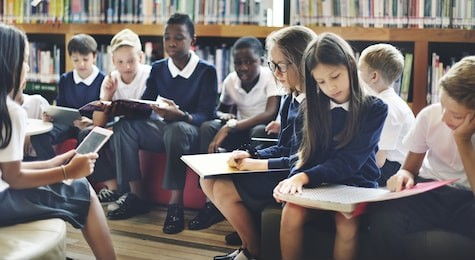
\includegraphics[scale=1]{images/school.jpg} 
\caption{Students in the library.}
\label{fig1: School Example}
\citep{archerapplications}

\end{figure}

We are familiar with students dropping out of schools based on different reasons. For example not everyone who joins graduate school makes it for graduation. The reasons for dropping out vary from one student to another. In some areas, most girls drop out in high school due to early pregnancies. What factors lead to early pregnancies? Peer influence, lack of proper guidance or adventure could be some of the reasons. Other reasons that could lead to school dropout may include illnesses, lack of school fees and psychological issues. 

We aim at reducing the number of school dropouts. We want to make predictions of a possible dropout before it actually happens. This will enable us to find a way to best assist the student as the Ministry of Education. Predictions are made based on statistics which means that we have to access the students data. We are dealing with all the schools for example high schools. This implies that the data should be stored in a central place. 

We do not fully trust the server. We also do not trust the other parties who may be using the server. No school is given access to another school's data. In some instances, the school may not have sufficient information to make a prediction. These are cases where for example, a sickness may be the cause of a dropout. This means that we require information from a hospital. We may also require information from different hospitals if the student has sought medication from more than one hospital. 

Another scenario is when a student drops out due to lack of school fees. We may need to check the financial status of the parents or guardian. This implies that banks and welfare services would be of great help. Different institutions therefore need to be integrated into the system. This makes it even more difficult. The schools may be reluctant to provide private information about the students due to laws that govern them. The central place where information is stored could be a potential target for attackers \citep{archerapplications}.

Homomorphic Encryption provides a solution to most of these problems. Data is encrypted before storage and computations are performed on the encrypted data. This ensures data sharing without breaking the laws. It also reduces the risk of an attack on the database. Data is encrypted in storage and also in transit. Different schools and sectors encrypt their data differently. They all use for instance, the RSA method, but have different public and private keys, therefore, no institution can decrypt another institution's data. As a result no single institution can access the whole data. We may also use secret sharing as an additional security measure to allow any computation. Secret Sharing as the name suggests, is the process whereby, authorization requires different pieces to be put together. The pieces are held by different people such that all combined can access the database, but an incomplete number of persons cannot. A good example is in a bank where a large transaction must be authorized by different people before it is processed. This builds the confidence  and a sense of ownership to the parties involved. We also ensure that the minimum number of persons  who can authorize involve persons who cannot collude. 

The first step is that different parties should approve access of a party to the database. After access is approved, a query is made to the server. The query is encrypted but the server knows the computation it is going to perform for example search function. Data about a specific student is accessed from different access points like a hospital and school. The data from these two places is encrypted differently and may be stored in different databases. If for example we get data from the school which shows that a student has been constantly sent home as a result of failure to pay school fees, we can query about the bank details. After the data is retrieved, it is then merged. A prediction is therefore made from the merged data based on the characteristics or the model used. Batch requests can also be made such that the dropout risk of students from an institution is performed simultaneously. 

This could be slow using a classical server and can even take days for a query to be processed. We therefore recommend a quantum computer as a server as it is fast and efficient. 


\section{Hospital Example}
Information about a person's health is usually sensitive and medical practitioners swear an oath of secrecy. This information should be protected at all costs to avoid leakage which may cause damage both to an individual and the institution itself. Researchers or the medical practitioners would want to use this data to conduct a research about a certain drug and its effect to the patients. They may also want to use the data for better planning or to predict an outcome. All these should be done while preserving the privacy of the patient.

\citet{archerapplications} describes a use case where the doctors record patients' details like blood group, genotype, signs and symptoms, lab test results, drug prescription and the efficiency of the medication administered. This is done over a period of time. The data is then encrypted and stored in the database where the server is not fully trusted as shown in figure \ref{fig1: Hosptial Example}. 
\begin{figure}[!h]
\center
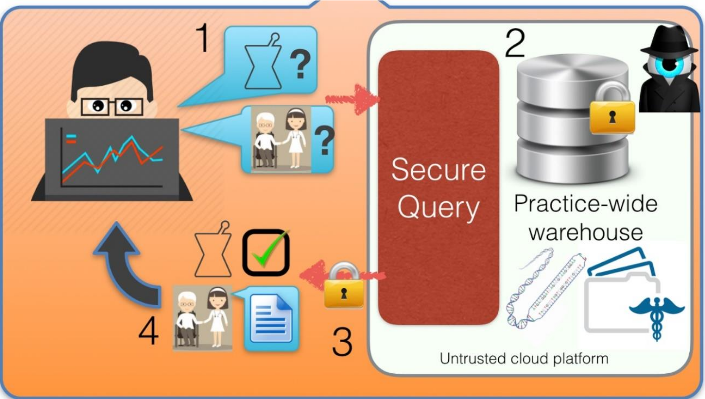
\includegraphics[scale=0.5]{images/hos.png} 
\caption{Hospital Example }
\label{fig1: Hosptial Example}
\citep{archerapplications}
\end{figure}

For cancer patients, the tumors differ from one patient to another. This implies that the treatments  also differ and patients may also react differently to the medication. The reaction may depend on things like the size of the tumor, allergic reactions and genes just to name a few. The details of different patients are already in the database. If a new patient visits the hospital the doctor queries the database based on the patient's details that are similar to those stored in the database, which may include signs and symptoms among others.
The query is encrypted but the computation is known to the server. After getting the results, the doctor decrypts and knows the best treatment to administer to the current patient based on different past results. This saves on time required to test the medication that would work on the patient. The patient requires to pay the bill after treatment. To pay the bill things like tests performed, diagnosis and prescription are exposed to the cashier. This could lead to leakage. Using homomorphic encryption, the amount could just be calculated and the payment made without exposing any additional details.

According to \citep{naehrig2011can}, the data stored about the patients can also be useful in several ways. Based on the patients data, functions would be computed to determine certain risks such as possibility of a re-infection and attacks like hypertension. Alerts are then sent to the doctor and the patient. The patient is hence in a position to act accordingly before the risk becomes a reality and safety precautions taken. This improves the efficiency of the services provided by the hospital. 

This argument is based on a classical client and a classical server. It can be implemented using a classical client and a quantum server as we have earlier seen the advantages of quantum computing over classical computing for instance speed and efficiency. This use case would therefore work best using Quantum Homomorphic Encryption.


The school and hospital use cases can also be implemented using Blind Quantum Computing. As we saw earlier, its main disadvantage is cost of implementation. This makes Quantum Homomorphic Encryption our most preferred option.



   